% Options for packages loaded elsewhere
\PassOptionsToPackage{unicode}{hyperref}
\PassOptionsToPackage{hyphens}{url}
%
\documentclass[
  english,
  man,floatsintext]{apa6}
\usepackage{lmodern}
\usepackage{amssymb,amsmath}
\usepackage{ifxetex,ifluatex}
\ifnum 0\ifxetex 1\fi\ifluatex 1\fi=0 % if pdftex
  \usepackage[T1]{fontenc}
  \usepackage[utf8]{inputenc}
  \usepackage{textcomp} % provide euro and other symbols
\else % if luatex or xetex
  \usepackage{unicode-math}
  \defaultfontfeatures{Scale=MatchLowercase}
  \defaultfontfeatures[\rmfamily]{Ligatures=TeX,Scale=1}
\fi
% Use upquote if available, for straight quotes in verbatim environments
\IfFileExists{upquote.sty}{\usepackage{upquote}}{}
\IfFileExists{microtype.sty}{% use microtype if available
  \usepackage[]{microtype}
  \UseMicrotypeSet[protrusion]{basicmath} % disable protrusion for tt fonts
}{}
\makeatletter
\@ifundefined{KOMAClassName}{% if non-KOMA class
  \IfFileExists{parskip.sty}{%
    \usepackage{parskip}
  }{% else
    \setlength{\parindent}{0pt}
    \setlength{\parskip}{6pt plus 2pt minus 1pt}}
}{% if KOMA class
  \KOMAoptions{parskip=half}}
\makeatother
\usepackage{xcolor}
\IfFileExists{xurl.sty}{\usepackage{xurl}}{} % add URL line breaks if available
\IfFileExists{bookmark.sty}{\usepackage{bookmark}}{\usepackage{hyperref}}
\hypersetup{
  pdftitle={Convolutional neural networks can decode eye movement data: A black box approach to predicting task from eye movements},
  pdflang={en-EN},
  pdfkeywords={deep learning, eye tracking, convolutional neural network, cognitive state, endogenous attention},
  hidelinks,
  pdfcreator={LaTeX via pandoc}}
\urlstyle{same} % disable monospaced font for URLs
\usepackage{graphicx,grffile}
\makeatletter
\def\maxwidth{\ifdim\Gin@nat@width>\linewidth\linewidth\else\Gin@nat@width\fi}
\def\maxheight{\ifdim\Gin@nat@height>\textheight\textheight\else\Gin@nat@height\fi}
\makeatother
% Scale images if necessary, so that they will not overflow the page
% margins by default, and it is still possible to overwrite the defaults
% using explicit options in \includegraphics[width, height, ...]{}
\setkeys{Gin}{width=\maxwidth,height=\maxheight,keepaspectratio}
% Set default figure placement to htbp
\makeatletter
\def\fps@figure{htbp}
\makeatother
\setlength{\emergencystretch}{3em} % prevent overfull lines
\providecommand{\tightlist}{%
  \setlength{\itemsep}{0pt}\setlength{\parskip}{0pt}}
\setcounter{secnumdepth}{-\maxdimen} % remove section numbering
% Make \paragraph and \subparagraph free-standing
\ifx\paragraph\undefined\else
  \let\oldparagraph\paragraph
  \renewcommand{\paragraph}[1]{\oldparagraph{#1}\mbox{}}
\fi
\ifx\subparagraph\undefined\else
  \let\oldsubparagraph\subparagraph
  \renewcommand{\subparagraph}[1]{\oldsubparagraph{#1}\mbox{}}
\fi
% Manuscript styling
\usepackage{upgreek}
\captionsetup{font=singlespacing,justification=justified}

% Table formatting
\usepackage{longtable}
\usepackage{lscape}
% \usepackage[counterclockwise]{rotating}   % Landscape page setup for large tables
\usepackage{multirow}		% Table styling
\usepackage{tabularx}		% Control Column width
\usepackage[flushleft]{threeparttable}	% Allows for three part tables with a specified notes section
\usepackage{threeparttablex}            % Lets threeparttable work with longtable

% Create new environments so endfloat can handle them
% \newenvironment{ltable}
%   {\begin{landscape}\begin{center}\begin{threeparttable}}
%   {\end{threeparttable}\end{center}\end{landscape}}
\newenvironment{lltable}{\begin{landscape}\begin{center}\begin{ThreePartTable}}{\end{ThreePartTable}\end{center}\end{landscape}}

% Enables adjusting longtable caption width to table width
% Solution found at http://golatex.de/longtable-mit-caption-so-breit-wie-die-tabelle-t15767.html
\makeatletter
\newcommand\LastLTentrywidth{1em}
\newlength\longtablewidth
\setlength{\longtablewidth}{1in}
\newcommand{\getlongtablewidth}{\begingroup \ifcsname LT@\roman{LT@tables}\endcsname \global\longtablewidth=0pt \renewcommand{\LT@entry}[2]{\global\advance\longtablewidth by ##2\relax\gdef\LastLTentrywidth{##2}}\@nameuse{LT@\roman{LT@tables}} \fi \endgroup}

% \setlength{\parindent}{0.5in}
% \setlength{\parskip}{0pt plus 0pt minus 0pt}

% \usepackage{etoolbox}
\makeatletter
\patchcmd{\HyOrg@maketitle}
  {\section{\normalfont\normalsize\abstractname}}
  {\section*{\normalfont\normalsize\abstractname}}
  {}{\typeout{Failed to patch abstract.}}
\makeatother
\shorttitle{Deep learning and eye tracking}
\author{Zachary J. Cole\textsuperscript{1}, Karl M. Kuntzelman\textsuperscript{1}, Michael D. Dodd\textsuperscript{1}, \& Matthew R. Johnson\textsuperscript{1}}
\affiliation{
\vspace{0.5cm}
\textsuperscript{1} University of Nebraska-Lincoln}
\authornote{

Correspondence concerning this article should be addressed to Zachary J. Cole, 238 Burnett Hall, Lincoln, NE 68588-0308. E-mail: z@neurophysicole.com}
\keywords{deep learning, eye tracking, convolutional neural network, cognitive state, endogenous attention\newline\indent Word count: X }
\usepackage{lineno}

\linenumbers
\usepackage{csquotes}
\usepackage{multirow}
\usepackage{graphicx}
\ifxetex
  % Load polyglossia as late as possible: uses bidi with RTL langages (e.g. Hebrew, Arabic)
  \usepackage{polyglossia}
  \setmainlanguage[]{english}
\else
  \usepackage[shorthands=off,main=english]{babel}
\fi

\title{Convolutional neural networks can decode eye movement data: A black box approach to predicting task from eye movements}

\date{}

\abstract{
We learned so deeply we incepted the inferred cogntive processes that underlie the inferred eye movement features.
}

\begin{document}
\maketitle

\section{}

The association between eye movements and mental activity is a fundamental topic of interest in attention research that has provided a foundation for developing a wide range of human assistive technologies. Foundational work by Yarbus (1967) showed that eye movement patterns appear to differ qualitatively depending on the task-at-hand (for a review of this work, see Tatler, Wade, Kwan, Findlay, \& Velichkovsky, 2010). A replication of this work by DeAngelus and Pelz (2009) shows that the differences in eye movements between tasks can be quantified, and appear to be generalizable. Technological advances and improvements in computing power have allowed researchers to determine the mental state underlying eye movement data, also known as the \enquote{inverse Yarbus process} (Haji-Abolhassani \& Clark, 2014). Current state-of-the-art machine learning and neural network algorithms are capable of identifying diagnostic patterns in the data for purposes of classification, but the inner workings of the resulting model solutions are difficult or impossible to interpret. Algorthims that provide uninterpretable solutions are referred to as \emph{black box} models. Dissections of black box models have been largely uninformative (Zhou, Bau, Oliva, \& Torralba, 2019), discouraging their implementation in basic research. Still, black box models provide a convenient solution for techonological applications such as human-computer interfaces (HCI; for a review, see Lukander, Toivanen, \& Puolamäki, 2017). While the internal operations of the model solutions used for HCI applications do not necessarily need to be interpretable to serve their purpose, Lukander et al. (2017) pointed out that \enquote{the black box nature of the resulting solution impedes generalizability, and makes applying methods across real life conditions more difficult} (p.~44). To ground these solutions, researchers guide black box decoding efforts by providing data and/or models with built-in theoretical assumptions. For instance, eye movement data is processed into meaningful aggregate properties such as fixations or saccades, or statistical features such as as fixation density, and the models used to decode these data are structured based on the current understanding of relevant cognitive or neurobiological processes (e.g., MacInnes, Hunt, Clarke, \& Dodd, 2018).

At this point, there is no clear evidence to support the notion that the standard theoretically grounded inferences actually enhance or clarify black box solutions beyond what could be inferred from an unconstrained model. Consider the case of Greene, Liu, and Wolfe (2012), who failed to classify task from commonly used aggregate eye movement features (i.e., number of fixations, mean fixation duration, mean saccade amplitude, percent of image covered by fixations) using three separate model architectures (see Table \ref{tab:previous-studies}. This led Greene and colleagues to question the robustness of Yarbus's (1967) findings, inspiring a slew of responses that successfully decoded the same dataset by aggregating the eye movements into different feature sets or implementing different model architectures (see Table \ref{tab:previous-studies}; i.e., Haji-Abolhassani \& Clark, 2014; Borji \& Itti, 2014; Kanan, Ray, Bseiso, Hsiao, \& Cottrell, 2014). The subsequent re-analyses of these data support Yarbus (1967) and the notion that mental state can be decoded using a variety of combinations of data features and model architectures. Despite using theoretically informed models to classify the data, these re-analyses do not explain the failures of Greene et al. (2012) anymore definitively than a black box approach.

Eye movements can only be differentiated to the extent that the cognitive processes underlying the tasks can be delineated (Król \& Król, 2018). Every task is associated with a unique set of cognitive processes (Coco \& Keller, 2014; Król \& Król, 2018). In some cases, the cognitive processes for different tasks may produce indistinguishable eye movement patterns. To distinguish the cognitive processes underlying task-evoked eye movements, some studies have chosen to classify tasks that rely on stimuli to prompt easily distinguishable eye movements, such as reading text and searching pictures (e.g., Henderson, Shinkareva, Wang, Luke, \& Olejarczyk, 2013). The eye movements elicited by salient stimulus features confound classifications of complex mental states because these eye movements are the consequence of a feature, or features, inherent to the stimulus rather than the goal directed shifting of attention (e.g., Henderson et al., 2013; Boisvert \& Bruce, 2016). Additionally, the distinct nature of exogenously elicited eye movements prompts decoding algorithms to prioritize these bottom-up patterns in the data over higher-level top-down effects (Borji \& Itti, 2014). This means that these models are identifying the type of information that is being processed, but are not necessarily reflecting the mental state of the individual observing the stimulus. Eye movements that are the product of bottom-up attentional processes can be reliably decoded, which is relevant for some HCI applications, but does not fit the explicit top-down nature of the inverse Yarbus problem.

The mental processes underlying eye movements elicited from top-down attentional processes remain relatively undefined. Prior evidence has shown that the task-at-hand is capable of producing distinguishable eye movement features such as the percentage of the stimulus fixated, total scan path length, total number of fixations, and the amount of time to the first saccade (Castelhano, Mack, \& Henderson, 2009; DeAngelus \& Pelz, 2009). Typical decoding accuracies within the context of determining task from eye movements typically range from chance performance to 59.64\% (see Table \ref{tab:previous-studies}). In one case, Coco and Keller (2014) categorized the same eye movement features used by Greene et al. (2012) with respect to the relative contribution of visual or linguistic components of three tasks (visual search, name the picture, name objects in the picture). By identifying the latent factors differentiating the tasks (i.e., relative linguistive or visual input), Coco and Keller (2014) was able to decode the eye movement data with 84\% accuracy. What stands out in the example of Coco and Keller (2014) is the use of a high level abstraction of the relevant task components that allowed for clear distinctions that were evident in the eye mvoement data. While this manipulation is remiscent of other experiments relying on the bottom-up influence of words and pictures (e.g., Henderson et al., 2013; Boisvert \& Bruce, 2016) the eye movements in the Coco and Keller (2014) tasks were entirely the product of top-down attentional processes. A conceptually similar follow-up to this study classified tasks along two spatial and semantic dimensions, resulting in 51\% classification accuracy (Król \& Król, 2018). A closer look at these results showed that the categories within the semantic dimension were consistently mixed up, suggesting that this level of distinction may require a more rich dataset, or a more powerful decoding algorithm. Altogether, this body of literature suggests that the use of tasks requiring distinct top-down attentional processes is an important factor to consider when classifying mental state from eye movement data.

\begin{table}[h]
    \centering
    \caption{Previous Studies}
    \label{tab:previous-studies}
    \begin{tabular}{p{.23\linewidth} p{.23\linewidth} p{.23\linewidth} p{.23\linewidth}}
        Study & Tasks & Model Architecture & Accuracy (Chance) \\
        \hline
        Greene et al. (2012) & memory, decade, people, wealth & linear discriminant, correlation, SVM & 25.9\% (25\%) \\
        Haji-Abolhassani \& James (2014)  & Greene et al. tasks & Hidden Markov Models & 59.64\% (25\%) \\
        Kanan et al. (2014) & Greene et al. tasks & multi-fixation pattern analysis & 37.9\% (25\%) \\
        Borji \& Itti (2014)  & Greene et al. tasks & kNN, RUSBoost & 34.34\% (25\%) \\
        Borji \& Itti (2014) & Yarbus tasks & kNN, RUSBoost & 24.21\% (14.29\%) \\
        Coco \& Keller (2014) & visual search, picture naming, object naming & MM, LASSO, SVM & 84\% (33\%) \\
        MacInnes et al. (2018) & view, memorize, search, preference & augmented Naive Bayes Network & 53.9\% (25\%) \\
        Król \& Król (2018) & people, indoors/outdoors, white/black, dot search & feed forward neural network & 51.4\% (25\%) \\
        \hline
    \end{tabular}
\end{table}

As shown in Table \ref{tab:previous-studies}, when eye movement data are prepared for classification, fixation and saccade statistics are typically aggregated along spatial or temporal dimensions, resulting variables such as fixation density or saccade amplitude (Castelhano et al., 2009; MacInnes et al., 2018; Mills, Hollingworth, Van der Stigchel, Hoffman, \& Dodd, 2011). The implementation of these statistical methods is meant to explicitly provide the decoding algorithm with characteristics of the eye movement data that are representative of theoretically relevant cognitive processes. For example, MacInnes et al. (2018) attempted to provide an algorithm with data assumed to be representative of inputs to the frontal eye fields. In some instances, such as the case of Król and Król (2018), grounding the data using theoretically driven aggregation methods may require sacrificing resolution in the dataset. This means that aggregating the data has the potential to wash out any fine-grained distinctinctions that could otherwise be detected. Data structures of any kind can only be decoded to the extent which the data is capable of representing differences between categories. Given the cognitive processes underlying distinct tasks are often overlapping (Coco \& Keller, 2014), decreasing the resolution of the data may actually limit the potential of the algorithm to classify the task.

The current state of the literature does not provide any coherent guidelines for determining what eye movement features are most meaningful, or what model architectures are most suited for determining mental state from eye movements. The theoretically informed models shown in Table \ref{tab:previous-studies} utilized a variety of eye movement features and model architectures, most of which were effective to a similar extent (with the exception of Greene et al., 2012). The complexities underlying these findings are not yet well-defined or understood. Basic research has provided a foundation of understanding, but has not provided any coherent guidelines to support generalizable applications of this research (Lukander et al., 2017). In an attempt to support practical applications of this body of research, the current study explored pragmatic solutions to the problem of classifying task from eye movement data.

The current study aimed to maximize the resolution of the data by submitting unprocessed x-coordinate, y-coordinate, and pupil size data to a convolutional neural network (CNN) model. Instead of transforming the data into theoretically defined meaningful units, we allowed the network to establish its own meaningful patterns in the data. CNNs have a natural propensity to develop low level feature detectors similar to primary visual cortex (e.g., Seeliger et al., 2018). For this reason, CNNs are commonly implemented for image classification. To test the possibility that the image data are better suited to the CNN classifier, the data will be decoded in raw timeline and image formats. To our knowledge, no study has attempted to address the inverse Yarbus problem using: (1) Non-aggregate data, (2) image data format, or (3) a CNN architecture. Given that CNN classification performance is robust to multidimensional, non-structured data, we expect the non-theoretically-constrained CNN architecture to decode both data types at levels consistent with the current state-of-the-art. Furthermore, we expect that despite evidence that black box approaches to the inverse Yarbus problem can be unreliable (Lukander et al., 2017), our initial findings will replicate when tested on an entirely separate dataset.

\section{Methods}

\subsection{Participants}

Two separate datasets were used to develop and test the deep CNN architecture. The two datasets were collected from two separate experiments, which we will refer to as Exploratory and Confirmatory. The participants for both datasets consisted of college students (Exploratory \emph{N} = 124; Confirmatory \emph{N} = 77) from the University of Nebraska-Lincoln who participated in exchange for class credit. Participants who took part in the exploratory experiment did not participate in the confirmatory experiment. All procedures and materials were approved by the University of Nebraska-Lincoln Institutional Review Board prior to data collection.

\subsection{Materials and Procedures}

Each participant viewed a series of scene images while carrying out a search, memorization, or rating task. For the search task, participants were instructed to find a \enquote{Z} or \enquote{N} embedded in the image. If the letter was found, the participants were instructed to press a button, which terminated the trial. For the memorization task, participants were instructed to memorize the image for a test that would take place when the task was completed. For the rating task, participants were asked to think about how they would rate the image on a scale from 1 (very unpleasant) to 7 (very pleasant). The participants were prompted for their rating immediately after viewing the image. The same materials were used in both experiments with a minor variation in the procedures. In the confirmatory experiment, participants were directed as to where search targets might appear in the image (e.g., on flat surfaces). No such instructions were provided in the exploratory experiment. In both experiments, trials were presented in one mixed block, and three separate task blocks. For the mixed block, the trial types were randomly intermixed within the block. For the three separate task blocks, each block consisted entirely of one of the three tasks (search, memorize, rate). Each trial was presented for 10 seconds. The inter-trial interval lasted seconds.

\subsection{Datasets}

Eye movements were recorded using an SR Research EyeLink II eye tracker with a sampling rate of 1000Hz. On some of the search trials, a probe was presented on the screen at six seconds. To equate the data from all three conditions, only the first six seconds of each trial were analyzed. Trials that were missing data were excluded before analysis. For both datasets, the trials were pooled across participants. After removing bad trials, the exploratory dataset consisted of 12,177 trials, and the confirmatory dataset consisted of 9,301 trials.

The raw x-coordinate, y-coordinate, and pupil size data collected at every sampling time point in the trial were used as inputs to the deep learning classifier. This data was also used to develop plot image datasets that were classified separately from the raw timeline datasets. For the plot image datasets, the timeline data for each trial were converted into scatterplot diagrams. The x- and y- coordinates and pupil size were used to plot each sample onto a scatterplot diagram (e.g., see Figure \ref{fig:ave-condition}). The coordinates were used to plot the location of the dot, pupil size was used to determine the relative size of the dot, and shading of the dot was used to indicate the time-course of the eye movements throughout the trial. The background of the plot images and first data point was white. The final data point was black. Each subsequent data point in between became incrementally darker until the final data point was reached. To ensure that every data point was fully represented within the scatterplot image, the pupil size value was divided by 10, and one unit was added to ensure the dot was at least one full unit. The plots were sized to match the dimensions of the data collection monitor (1024 x 768 pixels) then shrunk to (240 x 180 pixels) in an effort to reduce the dimensionality of the data.

\begin{figure}
\centering
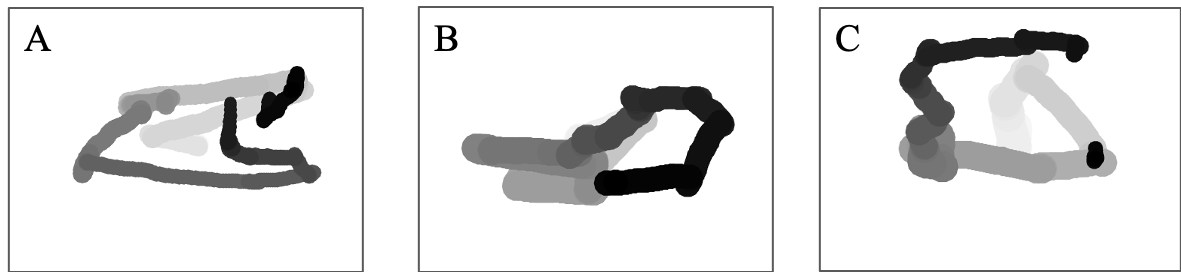
\includegraphics{images/cond_imgs.png}
\caption{\label{fig:ave-condition}The confusion matrices for the timeline format have shown the same pattern of results for the image set.}
\end{figure}

\subsubsection{Data Subsets.}

The full timeline dataset was structured into three columns representing the x- and y- coordinates, and pupil size for every sample collected in the first six seconds of each trial. To systematically assess the predictive value of each XYP (i.e., x-coordinates, y-coordinates, pupil size) component of the data, the timeline and image datasets were parcellated into subsets that excluded one of the components (i.e., XY\(\varnothing\), X\(\varnothing\)Y, \(\varnothing\)YP), or contained only one of the components (i.e., X\(\varnothing\varnothing\), \(\varnothing\)Y\(\varnothing\), \(\varnothing\varnothing\)P). For the timeline datasets, this means that the columns to be excluded in each data subset were replaced with zeros. The data were replaced with zeros because removing the columns would change the structure of the data. The same systematic parcellation process was carried out for the image dataset. See Figure \ref{fig:ave-subset} for an example of each of these image data subsets.

\begin{figure}
\centering
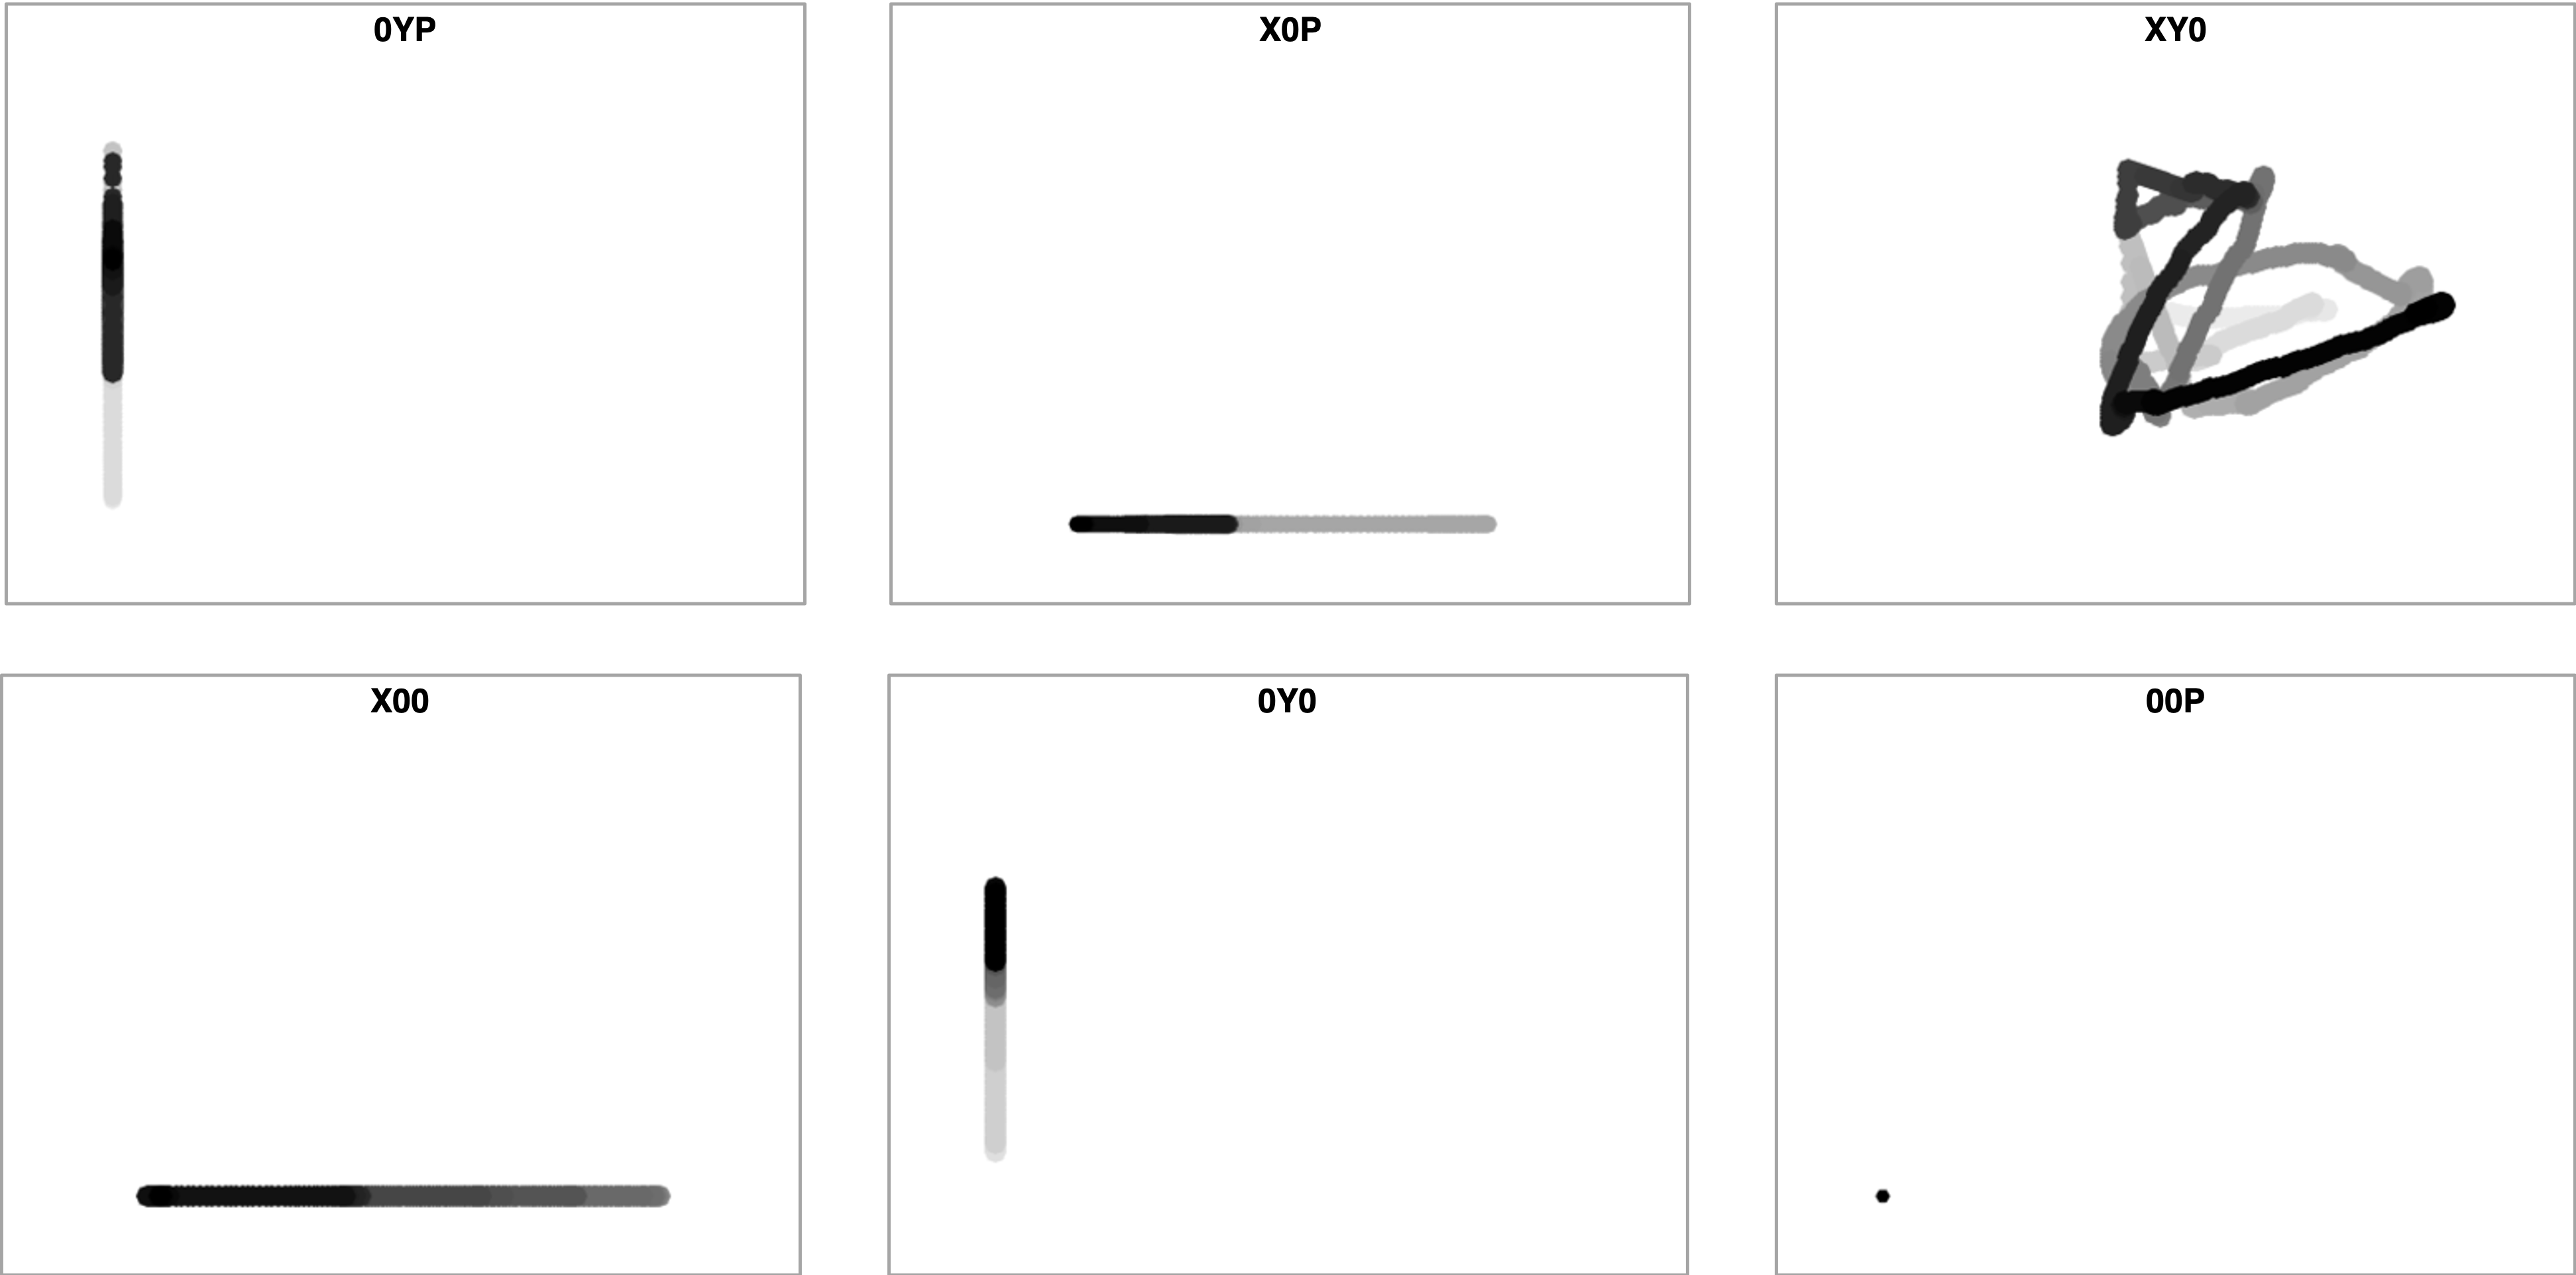
\includegraphics{images/subset_imgs.png}
\caption{\label{fig:ave-subset}The confusion matrices for the timeline format have shown the same pattern of results for the image set.}
\end{figure}

\subsection{Classification}

Deep CNN model architectures were implemented to classify the trials into search, memorize, or rate categories. Each model split the data into 70\% training, 15\% validation, and 15\% testing. Each network was run through 10 iterations of the data. Because the structure of the data generally plays a large role in CNN inferences, the differences in the structure of the timeline and image data formats required different CNN model architectures. The model architectures were developed with the intent of developing a generalizable model suited to the structure of the data. The development of these models was not guided by any formal theoretical assumptions regarding the patterns or features likely to be extracted by the classifier. The models were developed and tested on the exploratory dataset. Model parameters were adjusted until the classification accuracies no longer immproved. The model architecture with the highest classification accuracy on the exploratory dataset was tested independently on the confirmatory dataset. The model architectures used for the timeline and image datasets are shown in Figure \ref{fig:models}.

\begin{figure}
\centering
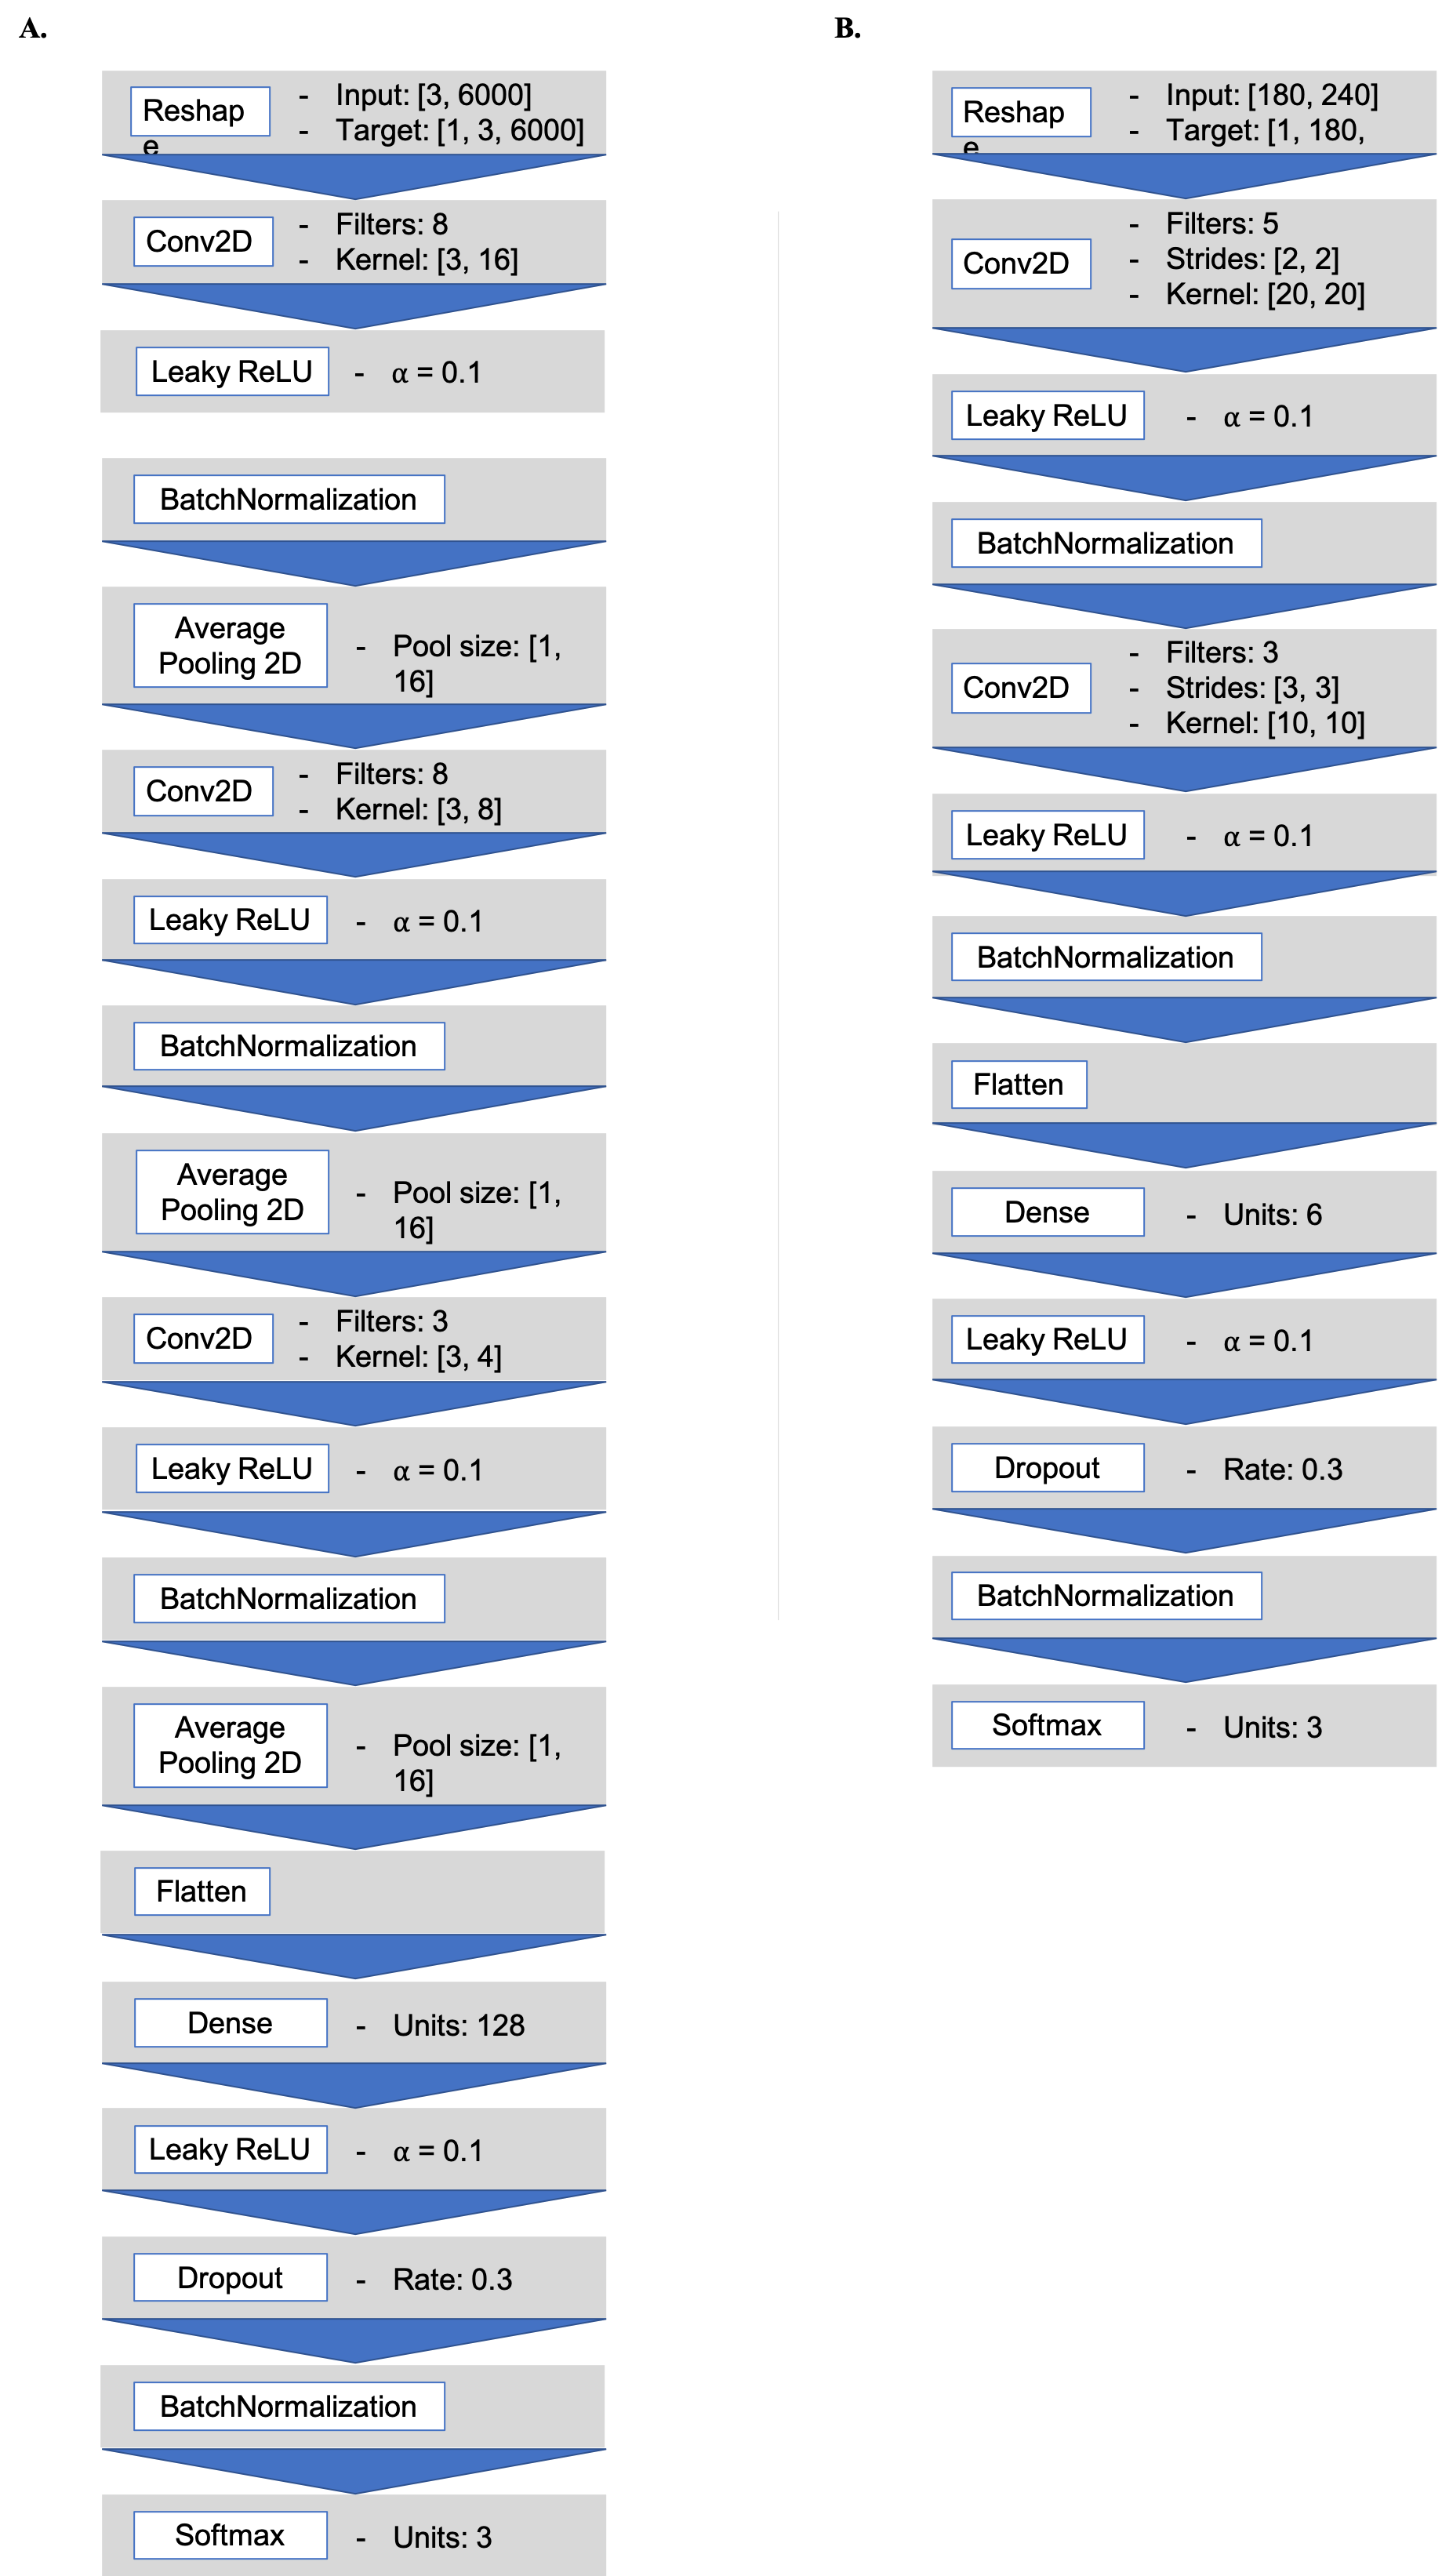
\includegraphics{images/models.png}
\caption{\label{fig:models}Differences in the structure of the timeline and image datasets meant the CNN models had to be different. A. Timeline model architecture. B. Image model architecture.}
\end{figure}

\subsection{Analysis}

Results for the CNN architecture that resulted in the highest accuracy on the exploratory dataset are reported below. For every dataset tested, a one-sample \emph{t}-test was used to compare the CNN accuracies against chance (33\%). The Shapiro-Wilk test of normality was conducted to test the normality for each dataset. When normality was assumed, the mean accuracy for that dataset was compared against chance using Student's one-sample \emph{t}-test. When normality could not be assumed, the median accuracy for that dataset was compared against chance using Wilcoxon's Signed Rank test.

To determine the relative value of the three components of the eye movement data, the data subsets were compared within the timeline and plot image data types. If classification accuracies were lower when the data was parcellated, the component that was removed was assumed to have some diagnostic contribution that the model was using to inform classification decisions. To determine the relative value of the contribution from each component, the accuracies from each subset with one component of the data removed were compared to the accuracies for the full dataset (XYP) using a one-way between-subjects Analysis of Variance (ANOVA). To further evaluate the decodability of each component independently, the accuracies from each subset containing only one component of the eye movement data were compared within a separate one-way between-subject ANOVA. All post-hoc comparisons were corrected using Tukey's \emph{HSD}.

\section{Results}

\subsection{Timeline Data Classification}
\subsubsection{Exploratory.}

Classification accuracies for the timeline data were well above chance (\emph{M} = .526, \emph{SD} = .018; \emph{t}(9) = 34.565, \emph{p} \textless{} .001). Accuracy for classifications of the data subsets were all better than chance (see Figure \ref{fig:timeline-parcellation-chance}). As shown in the confusion matrices displayed in Figure \ref{fig:timeline-conf-matrices}, the data subsets with lower overall classification accuracies almost always classified the Memorization condition at or below chance levels of accuracy. Misclassifications of the Memorization condition were split relatively evenly between the Search and Rate conditions.

\begin{figure}
\centering
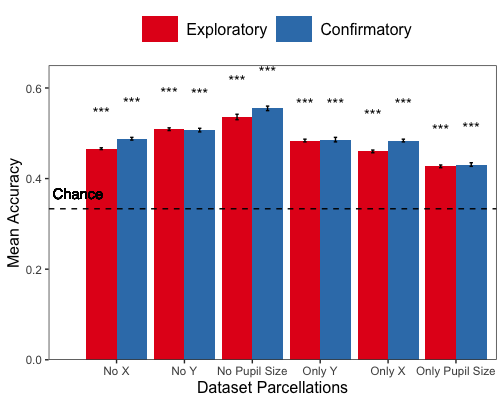
\includegraphics{results/r_code/timeline_parcellation_chance.png}
\caption{\label{fig:timeline-parcellation-chance}When overall accuracy was lower, the prediction accuracy of a dataset was lower.}
\end{figure}

\begin{figure}
\centering
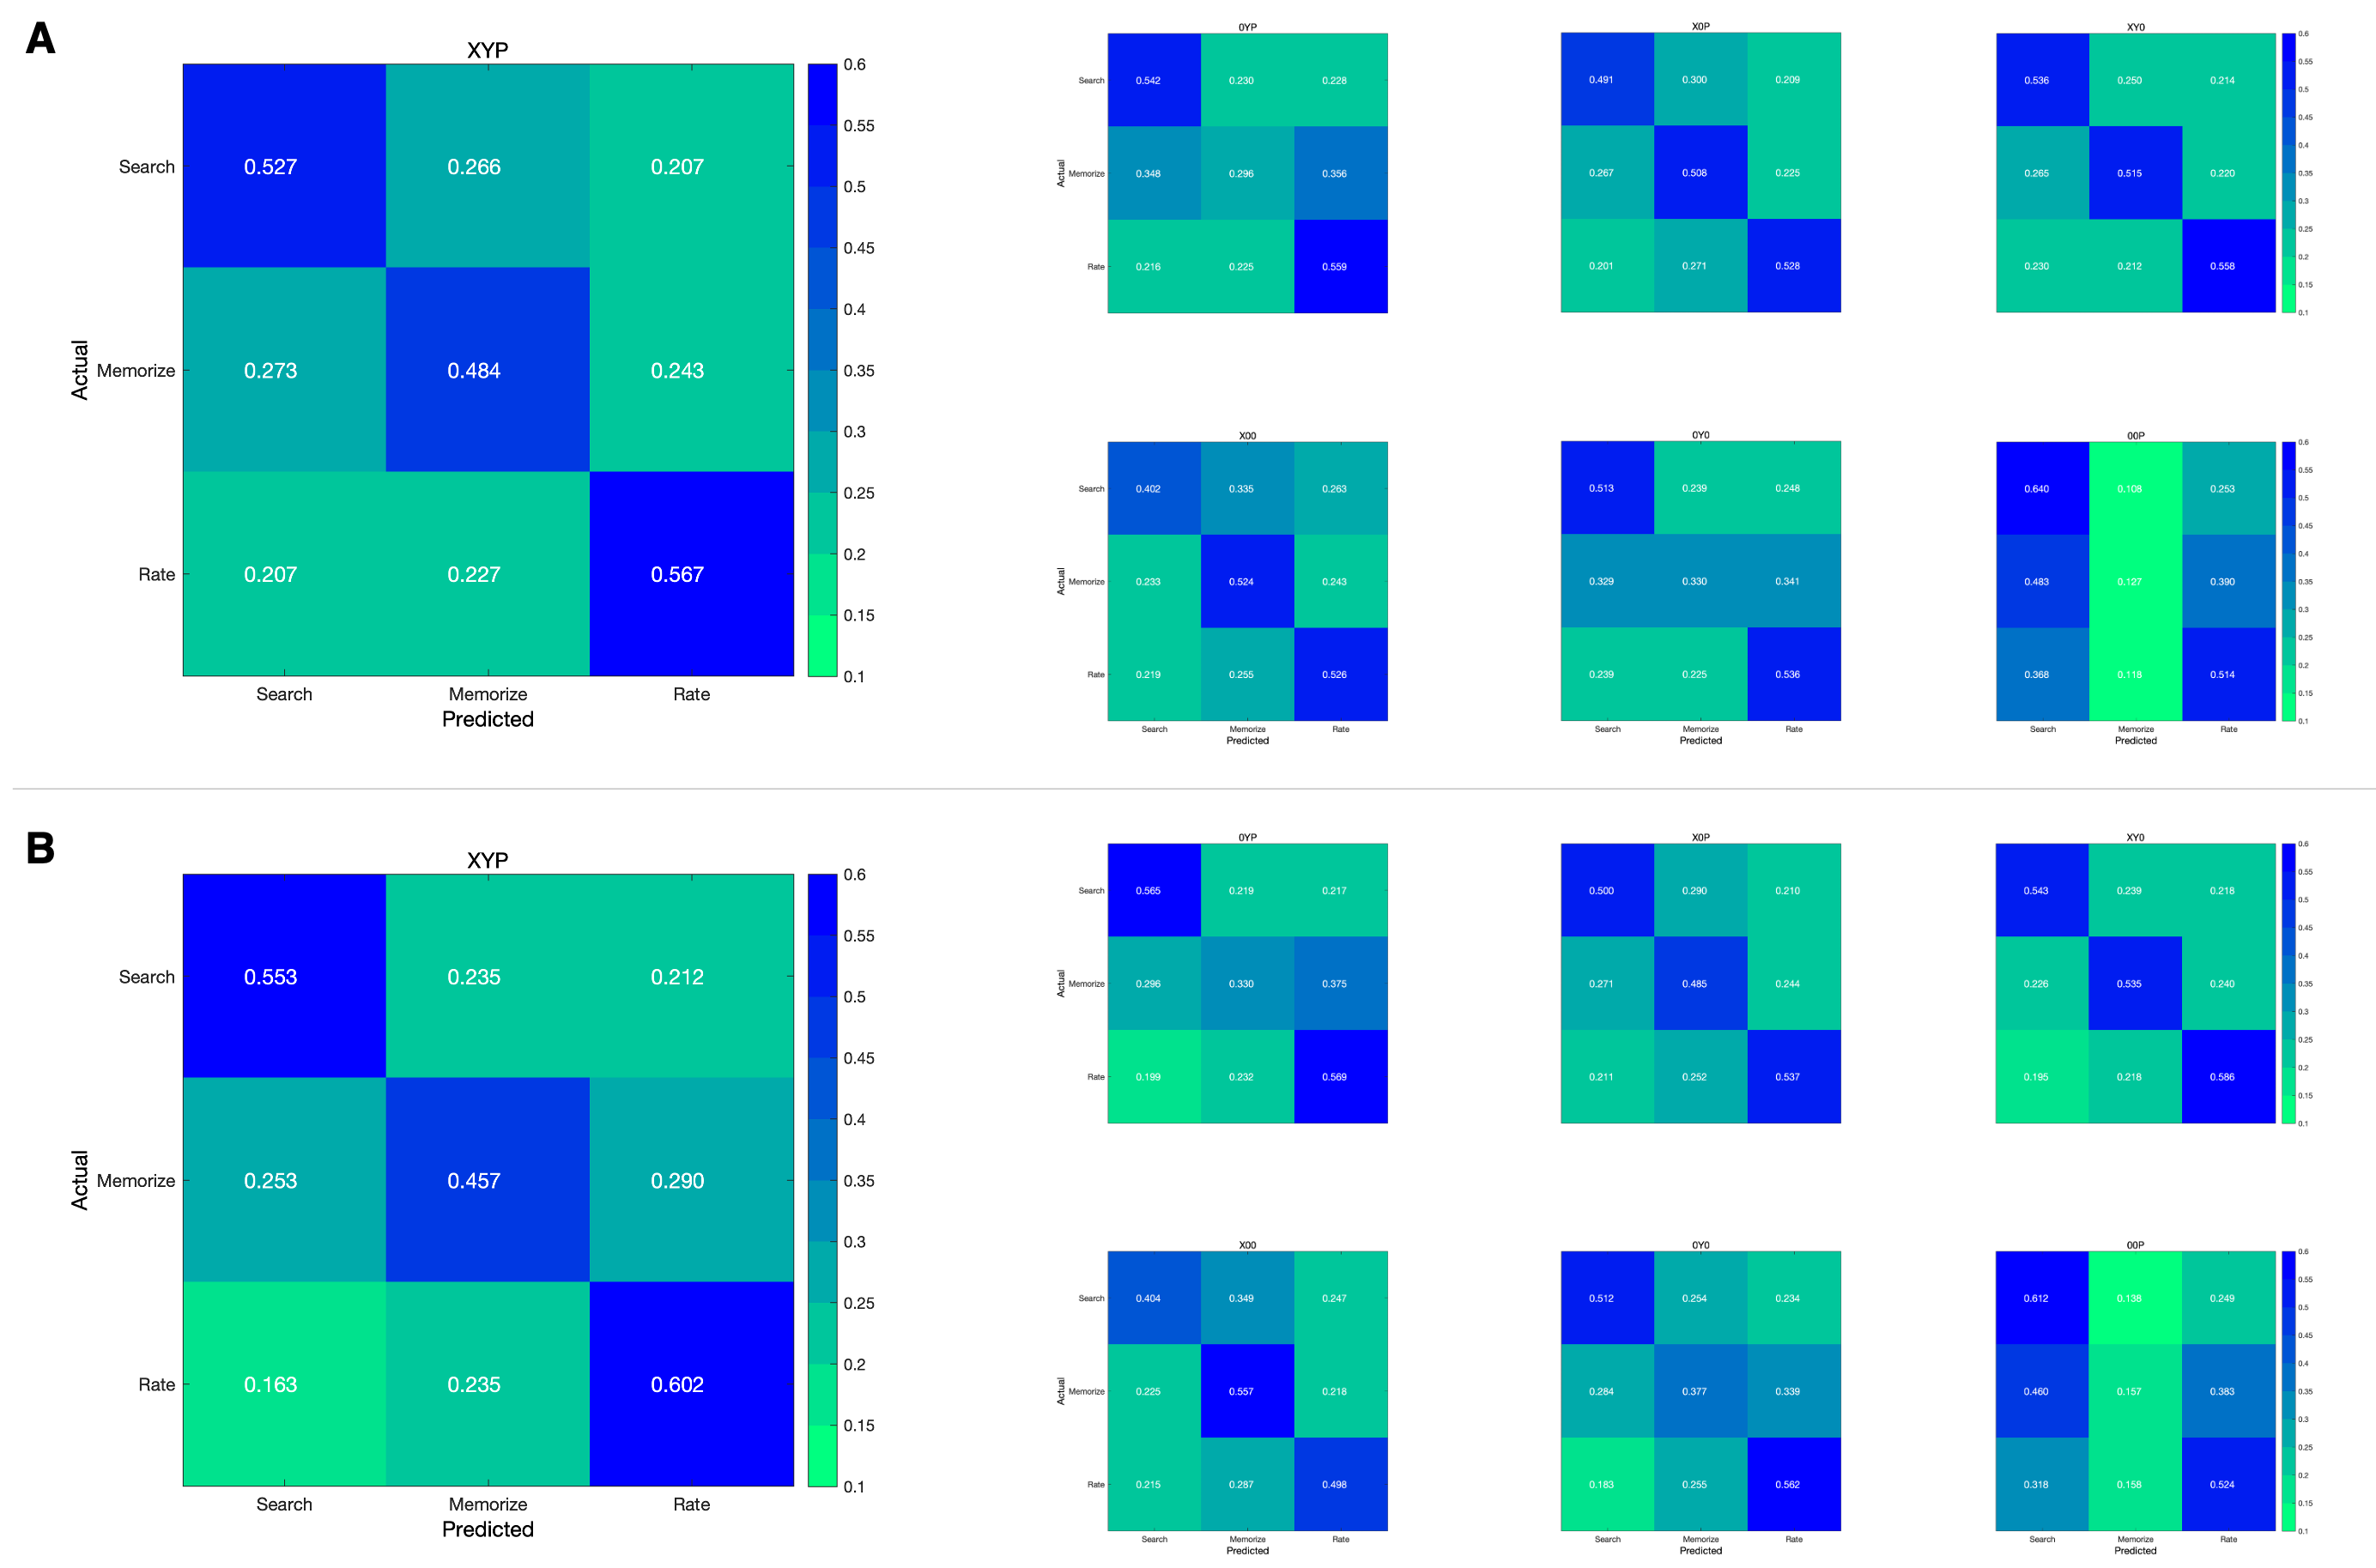
\includegraphics{images/timeline_conf_matrices.png}
\caption{\label{fig:timeline-conf-matrices}The confusion matrices for the timeline format have shown the same pattern of results for the image set.}
\end{figure}

There was a difference in classification accuracy for the XYP dataset and the subsets that had the pupil size, x-coordinate, and y-coordinate data systematically removed (\emph{F}\(_{(3, 36)}\) = 47.471, \emph{p} \textless{} .001, \textit{$\eta$}\(^{2}\) = 0.798). Post-hoc comparisons against the XYP dataset showed that classification accuracies were not affected by the removal of pupil size (\emph{t}\(_{(18)}\) = 1.635, \emph{p} = .372) or the y-coordinates (\emph{t}\(_{(18)}\) = 2.645, \emph{p} = .056). These null effects suggest that the pupil size and y-coordinate data were not informing classification judgments made by the CNN anymore than the data that was not removed. Classification for the \(\varnothing\)YP subset was lower than the XYP dataset (\emph{t}\(_{(18)}\) = 9.420, \emph{p} \textless{} .001), showing that these data were uniquely informative to the decoding model.

There was also a difference in classification accuracy for the X\(\varnothing\varnothing\), \(\varnothing\)Y\(\varnothing\), and \(\varnothing\varnothing\)P subsets (\emph{F}\(_{(2, 27)}\) = 75.145, \emph{p} \textless{} .001, \textit{$\eta$}\(^{2}\) = 0.848). Post-hoc comparisons show that classification accuracy for the \(\varnothing\varnothing\)P subset was lower than the X\(\varnothing\varnothing\) (\emph{t}\(_{(18)}\) = 12.213, \emph{p} \textless{} .001) and \(\varnothing\)Y\(\varnothing\) (\emph{t}\(_{(18)}\) = 7.026, \emph{p} \textless{} .001) subsets. Classification accuracy for the X\(\varnothing\varnothing\) subset was higher than the \(\varnothing\)Y\(\varnothing\) subset (\emph{t}\(_{(18)}\) = 5.187, \emph{p} \textless{} .001). These findings suggest that pupil size data was the variable least informative to classification decisions, while the x-coordinate data was the most informative.

\subsubsection{Confirmatory.}

Classification accuracy for the confirmatory timeline dataset was well above chance (\emph{M} = .537, \emph{SD} = 0.036, \emph{t}\(_{(9)}\) = 17.849, \emph{p} \textless{} .001). Classifications accuracies for the data subsets were also better than chance (see Figure \ref{fig:timeline-parcellation-chance}). Overall, there were some discrepancies in the pattern of results describing the relative contribution of the x- and y-coordinate data to the model (c.f., findings from the exploratory timeline dataset), but the general trend showing that pupil size was the least informative eye tracking data component remained stable in both datasets (see Table \ref{tab:parcellation-comparisons}). In concordance with the exploratory timeline dataset, the confusion matrices for these data revealed that the Memorization task was most often confused with the Search and Rate tasks (see Figure \ref{fig:timeline-conf-matrices}).

\begin{table}
    \centering
    \caption{Parcellation Comparisons}
    \label{tab:parcellation-comparisons}
    \begin{tabular}{p{0.12\textwidth} p{0.12\textwidth} p{0.12\textwidth} p{0.12\textwidth} p{0.12\textwidth} p{0.12\textwidth} p{0.12\textwidth}}
         & \multicolumn{3}{c}{Timeline} & \multicolumn{3}{c}{Image} \\
        \hline
        Comparison & \textit{t} & \textit{p} & Follows Pattern & \textit{t} & \textit{p} & Follows Pattern \\
        \cline{2-7}
        XYP \\
        $\hfill\varnothing$YP & 5.210 & < .001 & Y & 1.623 & .491 & Y \\
        $\hfill$X$\varnothing$P & 3.165 & .016 & N & 4.375 & < .001 & Y \\
        $\hfill$XY$\varnothing$ & 1.805 & .288 & Y & 1.557 & .532 & Y \\
        X$\varnothing\varnothing$ \\
        $\hfill\varnothing$Y$\varnothing$ & 0.495 & .874 & N & 2.807 & .204 & N \\
        $\hfill\varnothing\varnothing$ & 10.178 & < .001 & Y & 5.070 & < .001 & Y \\
        $\varnothing$Y$\varnothing$ \\
        $\hfill\varnothing\varnothing$P & 9.683 & < .001 & Y & 7.877 & < .001 & Y \\
        \hline
    \end{tabular}
\end{table}

To test the generalizability of the model to other eye tracking data, classification accuracies for the XYP exploratory and confirmatory timeline datasets were compared. The Shapiro-Wilk test for normality indicated that the exploratory (\emph{W} = 0.937, \emph{p} = .524) and confirmatory (\emph{W} = 0.884, \emph{p} = .145) datasets were normally distributed, but Levene's test indicated that the variances were not equal, \emph{F}\(_{(1, 18)}\) = 8.783, \emph{p} = .008. Welch's unequal variances \emph{t}-test did not show a difference between the two datasets, \emph{t}\(_{(13.045)}\) = 0.907, \emph{p} = .381, Cohen's \emph{d} = 0.406. These findings inidcate that the deep learning model decoded the exploratory and confirmatory timeline datasets equally well, but the confirmatory dataset classifications were less precise (as indicated by the standard deviations).

\subsection{Plot Image Classification}
\subsubsection{Exploratory.}

Classification accuracy for the plot image data were better than chance (\emph{M} = .436, \emph{SD} = .020, \emph{p} \textless{} .001), but were less accurate than the classifications for the exploratory timeline data (\emph{t}\(_{(18)}\) = 10.813, \emph{p} \textless{} .001). Accuracy for the classifications for all subsets of the plot image data except the \(\varnothing\varnothing\)P subset were better than chance (see Figure \ref{fig:img-parcellation-chance}. Following the pattern expressed by the timeline dataset, the confusion matrices showed that the Memorization condition was misclassified more often than the other conditions, and appeared to be evenly mis-identified as a Search or Rate condition (see Figure \ref{fig:img-conf-matrices}). The parsed plot image dataset classification accuracies were not compared to the parsed timeline dataset classification accuracies.

\begin{figure}
\centering
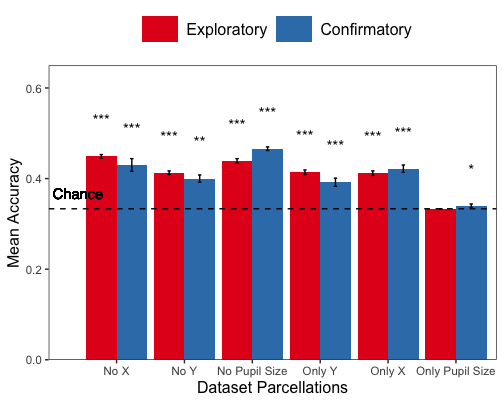
\includegraphics{results/r_code/img_parcellation_chance.png}
\caption{\label{fig:img-parcellation-chance}The confusion matrices for the timeline format have shown the same pattern of results for the image set.}
\end{figure}

\begin{figure}
\centering
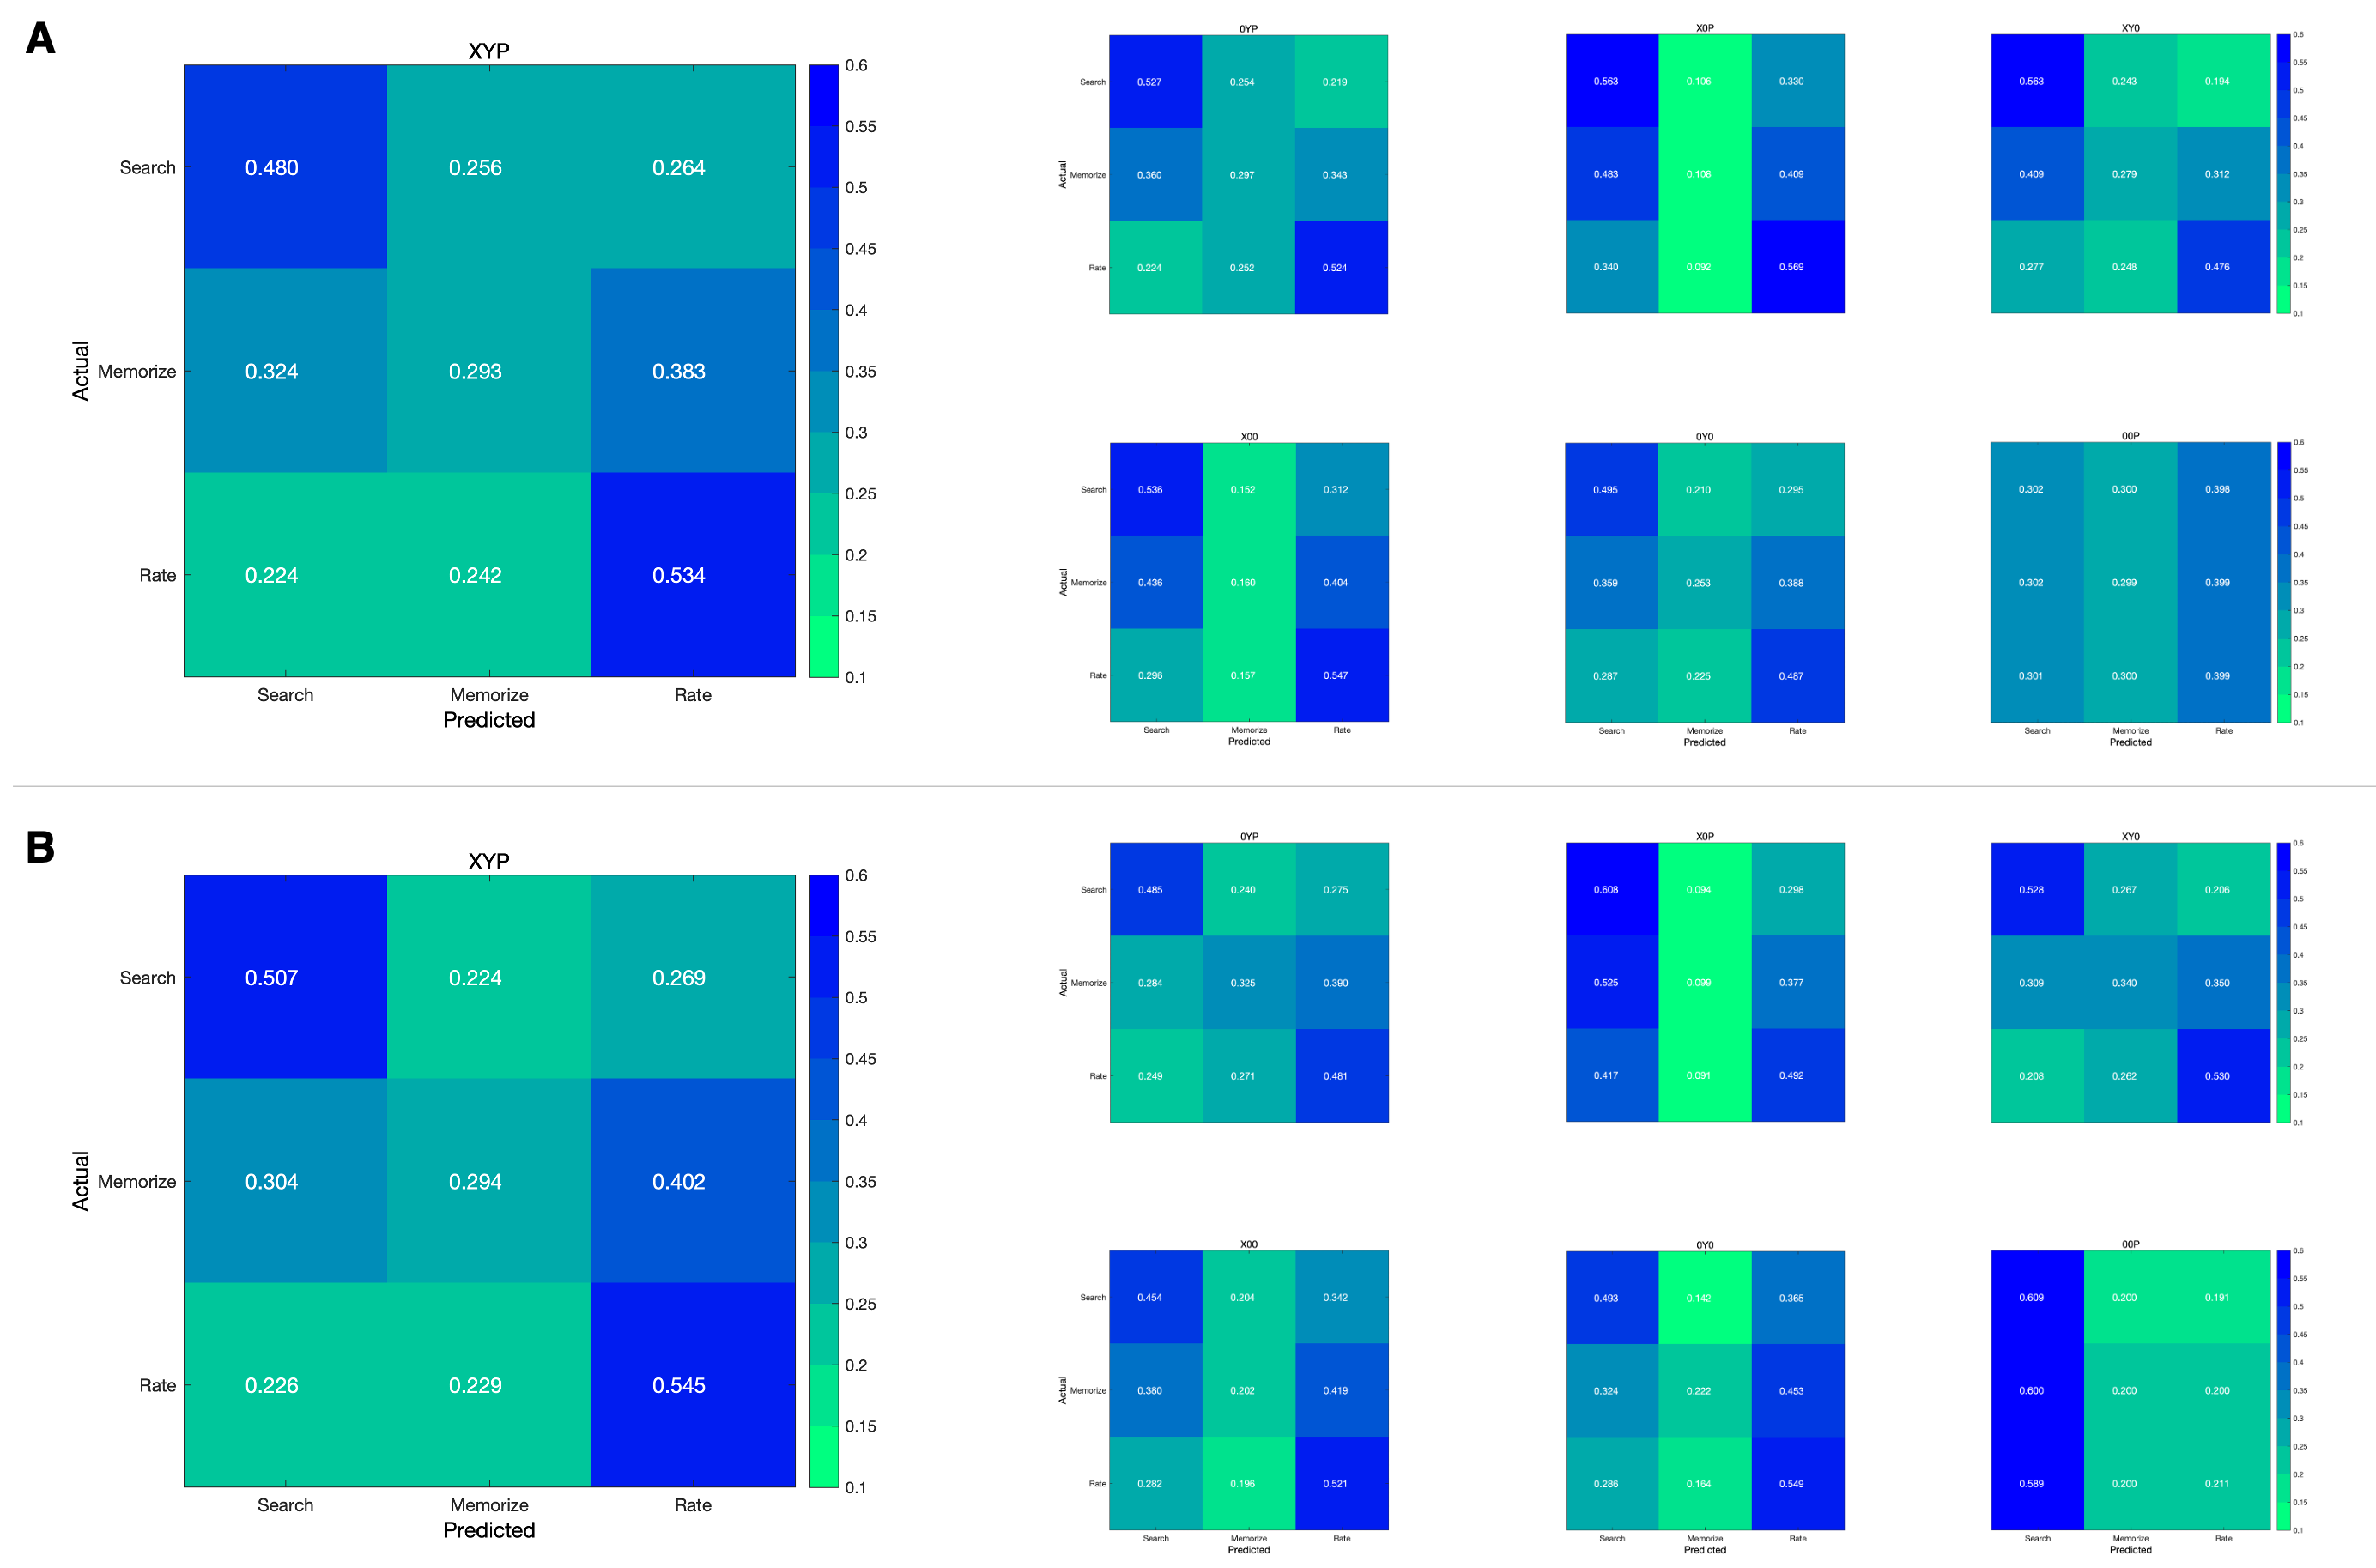
\includegraphics{images/img_conf_matrices.png}
\caption{\label{fig:img-conf-matrices}The confusion matrices for the timeline format have shown the same pattern of results for the image set.}
\end{figure}

There was a difference in classification accuracy for the XYP dataset and the data subsets (\emph{F}\(_{(4, 45)}\) = 7.093, \emph{p} \textless{} .001, \textit{$\eta$}\(^{2}\) = .387). Post-hoc comparisons showed that when compared to the XYP dataset, there was no effect of removing pupil size (\emph{t}\(_{(18)}\) = 0.474, \emph{p} = .989) or the x-coordinates (\emph{t}\(_{(18)}\) = 1.792, \emph{p} = .391), but classification accuracy was worse when the y-coordinates were removed (\emph{t}\(_{(18)}\) = 2.939, \emph{p} = .039).

There was also a difference in classification accuracy for the x\(\varnothing\varnothing\), \(\varnothing\)Y\(\varnothing\), and \(\varnothing\varnothing\)P subsets (\emph{F}\(_{(2, 17.993)}\) = 228.137, \emph{p} \textless{} .001, \textit{$\eta$}\(^{2}\) = .899). Because Levene's test revealed unequal variances between the groups (\emph{F}\(_{(2, 27)}\) = 3.815, \emph{p} = .035), the Welch correction was used to interpret the findings of this omnibus ANOVA. Post-hoc comparisons showed that there was no difference in classification accuracy for the X\(\varnothing\varnothing\) and \(\varnothing\)Yvarnothing subsets (\emph{t}\(_{(18)}\) = 0.423, \emph{p} = .906), but classification for the \(\varnothing\varnothing\)P subset were less accurate than the X\(\varnothing\varnothing\) (\emph{t}\({(18)}\) = 13.569, \emph{p} \textless{} .001) and \(\varnothing\)Y\(\varnothing\) (\emph{t}\(_{(18)}\) = 13.235, \emph{p} \textless{} .001) subsets.

\subsubsection{Confirmatory.}

Classification accuracy for the confirmatory image dataset was well above chance (\emph{M} = .449, \emph{SD} = 0.012, \emph{t}\(_{(9)}\) = 31.061, \emph{p} \textless{} .001), but was less accurate than the confirmatory timeline dataset classifications (\emph{t}\(_{(18)}\) = 11.167 \emph{p} \textless{} .001). Accuracy for classifications of the data subsets were also all better than chance (see Figure \ref{fig:img-parcellation-chance}. The confusion matrices followed the pattern showing that the Memorization condition was confused most often, and was relatively evenly mis-identified a Search or Rate trial (see Figure \ref{fig:img-conf-matrices}). As with the timeline data, there were discrepancies in the pattern of results describing the relative contribution of the x- and y-coordinate data to the model, but the general trend showing that pupil size data was the least informative to the model remained stable (see Table \ref{tab:parcellation-comparisons}).

To test the generalizability of the model, the classification accuracies for the XYP exploratory and confirmatory plot image datasets were compared. The independent samples \emph{t}-test showed that the deep learning model did equally well at classifying the exploratory and confirmatory plot image datasets, \emph{t}\(_{(18)}\) = 1.777, \emph{p} = .092, Cohen's \emph{d} = 0.795.

\section{Discussion}

The present study aimed to produce a practical and reliable example of a black box solution to the problem of the inverse Yarbus problem by classifying raw timeline and image data using a CNN model architecture. To our knowledge, this study was the first to provide a solution to determining mental state from eye movement data using each of the following: (1) Non-aggregated eye tracking data (x-coordinates, y-coordinates, pupil size), (2) timeline and image data formats (see Figure \ref{fig:ave-subset}), and (3) a \emph{black box} CNN architecture. This study probed the relative predictive value of the x-coordinate, y-coordinate, and pupil size components of the eye movement data using a CNN. The CNN was able to decode the image and timeline data better than chance, although only the timeline datasets were decoded with state-of-the-art accuracy. Datasets with lower classification accuracies were not able to differentiate the cognitive processes underlying the Memorization task from the cognitive processes underlying the Search and Rate tasks. Decoding subsets of the data revealed that pupil size was the least informative component of the eye movement data. This pattern of findings was consistent between the exploratory and confirmatory datasets.

Although several aggregate eye movement features have been tested as task predictors, to our knowledge, no other study has assessed the predictive value of the data format (viz., data in the format of an image). Our results suggest that although CNNs are robust image classifiers, eye movement data is decoded in the standard timeline format more effectively than in image format. This may be a consequence of the relative resolution of these data formats. Over the span of the trial (six seconds), the eye movements occasionally overlapped. When there was an overlap in the image data format, the more recent data points overwrote the older data points. This resulted in some data loss that did not occur when the data was represented in the standard timeline format. Despite the loss of overwritten data, the image format was still decoded with better than chance accuracy. To further examine the viability of classifying task from eye movement image datasets, future research might consider decoding 3-dimensional data formats, or more complex color combinations capable of representing overlapping data points.

When considering the superior performance of the timeline data (c.f., image data), we must also consider the differences in the model architectures. Because the structure of the timeline and image data formats were different, the models decoding those data structures also needed to be different. Both models were auditioned individually to the same extent on the Exploratory dataset before being tested on the confirmatory dataset. The exploratory and confirmatory pattern of results for both model architectures were the same, suggesting that these results are relatively stable. An appropriately developed CNN should be capable of learning any arbitrary fucntion, but given the atheoretical approach used to develop these models, there exists the possibility that an unknown model architecture exists which would produce equal or better classification accuracies for the image data format (c.f., timeline data format). Despite this possibility, the convergence of these findings with other studies (see Table \ref{tab:previous-studies}) suggests that the results of this study are approaching a ceiling for the potential predictive accuracy for eye tracking data.

Datasets with lower classification accuracies confused the Memorization condition with the Search and Rate conditions. This suggests that the eye movements associated with the memorization task are likely indicative of underlying cognitive processes that are shared by the Search and Rate tasks. Previous research (i.e., Król \& Król, 2018) has attributed the inability to differentiate one condition from the others to a lack of clarity in the data. This attribution is supported in the data by evidence that the subset data, with fewer defined variables, classified the memorization task less accurately than the other tasks. In cases when the subsets were decoded equally as well as the main dataset, the Memorize condition was classified as accurately as the other conditions.

When determining the relative contributions of the the eye movement features used in this study (x-coordinates, y-coordinates, pupil size), pupil size data was consistently the least informative. When pupil size was removed from the exploratory and confirmatory timeline and image datasets, classification accuracy remained stable (c.f., XYP dataset). Furthermore, classification of the \(\varnothing\varnothing\)P subset was the lowest of all of the data subsets, and in one instance, was no better than chance.

The findings from the current study support the notion that black box CNNs are a viable approach to determining task from eye movement data. In a recent review, Lukander et al. (2017) expressed concern regarding the lack of generalizability of black box approaches when decoding eye movement data. The current study showed a consistent pattern of results for the XYP timeline and image datasets, but some inconsistency in the pattern of results for the x- and y- coordinate subset comparisons. These findings suggest that the decoding decisions for the x- and y- coordinate subsets were less reliable, and may not be generalizable. This lack of reliability may be a product of overlap in the cognitive processes underlying the three tasks. Becuase the data subsets are all missing at least one dimension of the data, this lack of reliability may be attributable to the loss of meaningful data in the subsets. When the data provide fewer meaningul distinctions, more fine-grained inferences are required to distinguish the tasks. As shown by Coco and Keller (2014), eye movement data can be more effectively decoded when the cognitive processes underlying the tasks are explicitly distinguishable. While the cognitive processes distinguishing memorizing, searching, or rating an image are intuitively different, the eye movements elicited from these cognitive processes are not easily differentiated. To correct for potential mismatches between the level of distinction provided by the data and the level of distinction required for accurate and reliable classification of the data, future research could more definitively conceptualize the cognitive processes underlying the task-at-hand.

In reality, the level of abstraction differentiating the tasks-at-hand will depend on the application. Classifying mental state from eye movement data is often carried out in an effort to advance technology to improve educational outcomes, strengthen the independence of physically and mentally handicapped individuals, or improve HCI's {[}koocahakiPredictingIntentionEye2018{]}. To this end, the use of consistently effective and efficient black box solutions can be justified.

Given the questionable reliability and generalizability surrounding the \emph{black box} nature of CNN classification, the current study first tested models on an exploratory dataset, then confirmed the outcome using a second unrelated dataset. Overall, the findings appear stable and generalizable. Although the timeline data outperformed the image data format, future studies that incorporate stimulus features have the potential to provide a solution to determining task from eye movement data that surpasses the current state-of-the-art. According to Bulling, Weichel, and Gellersen (2013), incorporating stimulus feature information into the dataset may provide information is diagnostic beyond decoding spatial location data alone. Alternatively, Borji and Itti (2014) suggested that accounting for salient features in the the stimulus might leave little to no room for the classifier to consider mental state. If the goal is to improve classification accuracies for real-life applications, the inclusion of stimulus feature information in addition to the eye movement data may boost the classification accuracy of image data beyond that of the timeline data.

\hypertarget{section}{%
\subsection{\texorpdfstring{\newpage}{}}\label{section}}

\hypertarget{nocite-yarbuseyemovementsvision1967}{%
\subsection{nocite: : Yarbus (1967)}\label{nocite-yarbuseyemovementsvision1967}}

\begingroup
\setlength{\parindent}{-0.5in}
\setlength{\leftskip}{0.5in}

\hypertarget{refs}{}
\leavevmode\hypertarget{ref-boisvertPredictingTaskEye2016}{}%
Boisvert, J. F. G., \& Bruce, N. D. B. (2016). Predicting task from eye movements: On the importance of spatial distribution, dynamics, and image features. \emph{Neurocomputing}, \emph{207}, 653--668. \url{https://doi.org/10.1016/j.neucom.2016.05.047}

\leavevmode\hypertarget{ref-borjiDefendingYarbusEye2014a}{}%
Borji, A., \& Itti, L. (2014). Defending Yarbus: Eye movements reveal observers' task. \emph{Journal of Vision}, \emph{14}(3), 29--29. \url{https://doi.org/10.1167/14.3.29}

\leavevmode\hypertarget{ref-bullingEyeContextRecognitionHighlevel2013}{}%
Bulling, A., Weichel, C., \& Gellersen, H. (2013). EyeContext: Recognition of high-level contextual cues from human visual behaviour. In \emph{Proceedings of the SIGCHI Conference on Human Factors in Computing Systems - CHI '13} (p. 305). Paris, France: ACM Press. \url{https://doi.org/10.1145/2470654.2470697}

\leavevmode\hypertarget{ref-castelhanoViewingTaskInfluences2009}{}%
Castelhano, M. S., Mack, M. L., \& Henderson, J. M. (2009). Viewing task influences eye movement control during active scene perception. \emph{Journal of Vision}, \emph{9}(3), 6--6. \url{https://doi.org/10.1167/9.3.6}

\leavevmode\hypertarget{ref-cocoClassificationVisualLinguistic2014}{}%
Coco, M. I., \& Keller, F. (2014). Classification of visual and linguistic tasks using eye-movement features. \emph{Journal of Vision}, \emph{14}(3), 11--11. \url{https://doi.org/10.1167/14.3.11}

\leavevmode\hypertarget{ref-deangelusTopdownControlEye2009}{}%
DeAngelus, M., \& Pelz, J. B. (2009). Top-down control of eye movements: Yarbus revisited. \emph{Visual Cognition}, \emph{17}(6-7), 790--811. \url{https://doi.org/10.1080/13506280902793843}

\leavevmode\hypertarget{ref-greeneReconsideringYarbusFailure2012a}{}%
Greene, M. R., Liu, T., \& Wolfe, J. M. (2012). Reconsidering Yarbus: A failure to predict observers' task from eye movement patterns. \emph{Vision Res}, \emph{62}, 1--8. \url{https://doi.org/10.1016/j.visres.2012.03.019}

\leavevmode\hypertarget{ref-haji-abolhassaniInverseYarbusProcess2014}{}%
Haji-Abolhassani, A., \& Clark, J. J. (2014). An inverse Yarbus process: Predicting observers' task from eye movement patterns. \emph{Vision Research}, \emph{103}, 127--142. \url{https://doi.org/10.1016/j.visres.2014.08.014}

\leavevmode\hypertarget{ref-hendersonPredictingCognitiveState2013a}{}%
Henderson, J. M., Shinkareva, S. V., Wang, J., Luke, S. G., \& Olejarczyk, J. (2013). Predicting Cognitive State from Eye Movements. \emph{PLoS ONE}, \emph{8}(5), e64937. \url{https://doi.org/10.1371/journal.pone.0064937}

\leavevmode\hypertarget{ref-kananPredictingObserverTask2014}{}%
Kanan, C., Ray, N. A., Bseiso, D. N. F., Hsiao, J. H., \& Cottrell, G. W. (2014). Predicting an observer's task using multi-fixation pattern analysis. In \emph{Proceedings of the Symposium on Eye Tracking Research and Applications - ETRA '14} (pp. 287--290). Safety Harbor, Florida: ACM Press. \url{https://doi.org/10.1145/2578153.2578208}

\leavevmode\hypertarget{ref-krolRightLookJob2018}{}%
Król, M. E., \& Król, M. (2018). The right look for the job: Decoding cognitive processes involved in the task from spatial eye-movement patterns. \emph{Psychological Research}. \url{https://doi.org/10.1007/s00426-018-0996-5}

\leavevmode\hypertarget{ref-lukanderInferringIntentAction2017}{}%
Lukander, K., Toivanen, M., \& Puolamäki, K. (2017). Inferring Intent and Action from Gaze in Naturalistic Behavior: A Review. \emph{International Journal of Mobile Human Computer Interaction}, \emph{9}(4), 41--57. \url{https://doi.org/10.4018/IJMHCI.2017100104}

\leavevmode\hypertarget{ref-macinnesjosephGenerativeModelCognitive2018}{}%
MacInnes, W., Joseph, Hunt, A. R., Clarke, A. D. F., \& Dodd, M. D. (2018). A Generative Model of Cognitive State from Task and Eye Movements. \emph{Cognitive Computation}, \emph{10}(5), 703--717. \url{https://doi.org/10.1007/s12559-018-9558-9}

\leavevmode\hypertarget{ref-millsExaminingInfluenceTask2011}{}%
Mills, M., Hollingworth, A., Van der Stigchel, S., Hoffman, L., \& Dodd, M. D. (2011). Examining the influence of task set on eye movements and fixations. \emph{Journal of Vision}, \emph{11}(8), 17--17. \url{https://doi.org/10.1167/11.8.17}

\leavevmode\hypertarget{ref-seeligerConvolutionalNeuralNetworkbased2018}{}%
Seeliger, K., Fritsche, M., Güçlü, U., Schoenmakers, S., Schoffelen, J.-M., Bosch, S. E., \& van Gerven, M. A. J. (2018). Convolutional neural network-based encoding and decoding of visual object recognition in space and time. \emph{NeuroImage}, \emph{180}, 253--266. \url{https://doi.org/10.1016/j.neuroimage.2017.07.018}

\leavevmode\hypertarget{ref-tatlerYarbusEyeMovements2010}{}%
Tatler, B. W., Wade, N. J., Kwan, H., Findlay, J. M., \& Velichkovsky, B. M. (2010). Yarbus, Eye Movements, and Vision. \emph{I-Perception}, \emph{1}(1), 7--27. \url{https://doi.org/10.1068/i0382}

\leavevmode\hypertarget{ref-yarbusEyeMovementsVision1967}{}%
Yarbus, A. (1967). Eye Movements and Vision. Retrieved January 24, 2019, from \url{http://wexler.free.fr/library/files/yarbus\%20(1967)\%20eye\%20movements\%20and\%20vision.pdf}

\leavevmode\hypertarget{ref-zhouComparingInterpretabilityDeep2019}{}%
Zhou, B., Bau, D., Oliva, A., \& Torralba, A. (2019). Comparing the Interpretability of Deep Networks via Network Dissection. In W. Samek, G. Montavon, A. Vedaldi, L. K. Hansen, \& K.-R. Müller (Eds.), \emph{Explainable AI: Interpreting, Explaining and Visualizing Deep Learning} (pp. 243--252). Cham: Springer International Publishing. \url{https://doi.org/10.1007/978-3-030-28954-6_12}

\endgroup

\end{document}
